\documentclass[a4paper,fontsize=14pt]{article}

\usepackage{cmap} %поиск в PDF
\usepackage[T2A]{fontenc}
\usepackage[utf8]{inputenc}
\usepackage[russian]{babel}
\usepackage[14pt]{extsizes}
\usepackage[left=35mm,right=10mm,
top=20mm,bottom=20mm,bindingoffset=0cm]{geometry}
\usepackage{listings}
\lstset{language=Python}
\lstset{frame=lines}
\lstset{caption={Insert code directly in your document}}
\lstset{label={lst:code_direct}}
\lstset{basicstyle=\footnotesize}

\usepackage[tocflat]{tocstyle}

\usepackage{graphicx}
\graphicspath{ {./images/} }


\begin{document}
	
	\begin{titlepage}
		\newpage
		
		\begin{center}
			Санкт-Петербургский политехнический университет Петра Великого \\
			Институт прикладной математики и механики \\
			\textbf{Высшая школа теоретической механики}
		\end{center}
		
		\vspace{10em}
		
		\begin{center}
			\Large{\textbf{Лабораторная работа №2}} \\
			Уравнение колебаний струны. Вариант 6. \\
		\end{center}
		
		\vspace{20em}
		
		
		
		\newbox{\lbox}
		\savebox{\lbox}{\hbox{Е.Ю. Витохин}}
		\newlength{\maxl}
		\setlength{\maxl}{\wd\lbox}
		\hfill\parbox{12cm}{
			\hspace*{5cm}\hspace*{-5cm}Студент:\hfill\hbox to\maxl{А.А. Дурнев\hfill}\\
			\hspace*{5cm}\hspace*{-5cm}Преподаватель:\hfill\hbox to\maxl{Е.Ю.Витохин}\\
			\\
		}
		
		
		\vspace{\fill}
		
		\begin{center}
			Санкт-Петербург \\2020
		\end{center}
		
	\end{titlepage}
	
	\tableofcontents
	
	\newpage
	
	\section{Постановка задачи}
	
	Необходимо, используя метод конечных разностей, составить решение уравнения колебания струны вида: \\
	
	\begin{equation}
	\frac{\partial^2 U}{\partial t} = \frac{\partial^2 U}{\partial x^2}, \; x \in [0; 1], \; t \in [0; 0.5]
	\end{equation}

	где $x$ - пространственная координата, $t$ - время.\\
	
	Граничные условия:
	
	\begin{equation}
	U(0,t)=0, \; T(1;t)=1.2(t+1)
	\end{equation}
	
	Начальные условия:
	\begin{equation}
	U(x, 0) = (x+0.2)sin(\frac{\pi x}{2}), \; \dot{U}(x,0)=1+x^2
	\end{equation}
	
	
	Для численного решения уравнения будет использоваться явная схема метода конечных разностей. Решением будет являться сеточная функция $U(x, t)$ - распределение перемещения, заданная на двумерной сетке.

	\section{Описание метода}
	
	Задаём сетки по осям $x$ и $t$:
	\begin{equation}
		t_k = k\Delta t,\; k=0,\dots,K	
	\end{equation}
	\begin{equation}
		x_i=ih, \; i=0,\dots,N
	\end{equation}
	
	$\Delta t$ и $h$ - шаг сетки по осям $t$ и $x$ соответственно, $K$ и $N$ - количество узлов сетки по осям $t$ и $x$ соответственно. \\
	
	Производные приближаем конечными разностями: \\
	\begin{equation}
		\frac{\partial^2 U(t_k, x_i)}{\partial t} = \frac{U(t_{k+1}, x_i) - 2U(t_k, x_i) + U(t_{k-1}, x_i)}{\Delta t^2}
	\end{equation}
	\begin{equation}
		\frac{\partial^2 U(t_k, x_k)}{\partial x^2} = \frac{U(t_k, x_{i-1}) - 2U(t_k, x_k) + U(t_k, x_{i+1})}{h^2}
	\end{equation} \\
	
	Используя уравнение Даламбера выводим рекурентное соотношение: \\
	
	\begin{equation}
	\frac{\partial^2 U(t_k, x_k)}{\partial x^2} - \frac{\partial^2 U(t_k, x_i)}{\partial t} = 0
	\end{equation} \\
	
	Подставляем (6) и (7) в (8) и получаем:
	
	\begin{equation}
		U(t_{k+1}, x_i) = (U(t_k, x_{i+1}) - 2U(t_k, x_i) + U(t_k, x_{i-1})) \frac{\Delta t^2}{h^2} + 2U(t_k, x_i) - U(t_{k-1}, x_i)
	\end{equation} \\
	
	Выражение (8) позволяется получать значение функции $U(x, t)$ на $k+1$ слое,использую значения с $k$-ого и $k-1$-го слоя сетки (схема-крест). Начальные значения на сетке инициа-лизируются при помощи (2) и (3).\\
	
	Чтобы заполнить 1-ый слой по времения используем соотношение: \\
	
	\begin{equation}
	U(t_1, x_i) = U(0,x_i) + \dot{U}(0,x_i)\Delta t + \frac{\Delta t^2}{2h^2}(U(0, x_{i+1}) - 2U(0, x_i) + U(0, x_{i-1}))
	\end{equation} \\
	
	Оно позволяет нам сохранить 2 порядок точности метода. 
	
	
	\section{Описание результатов}
	
	В качестве шагов для сетки берём: $\Delta t = 0.01, \; h = 0.1$. Полученное решение представлено на Рис.1: \\
	
	\begin{figure}[h]
		\center{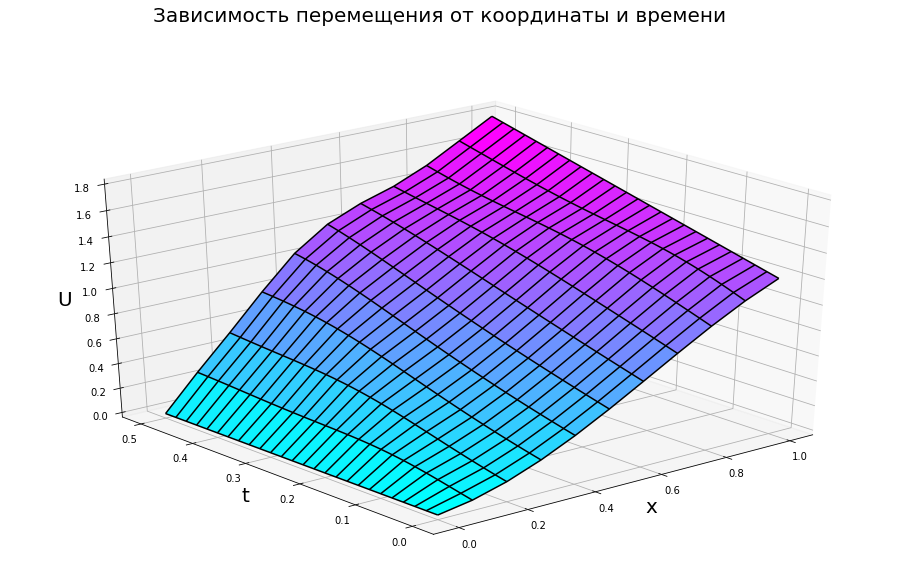
\includegraphics[scale=0.55]{pic1.png}}
		\label{pic1}
		\caption{}
	\end{figure}
	
	\newpage
	
	Изобразим проекции решения на плоскости:
	
	\begin{figure}[h]
		\center{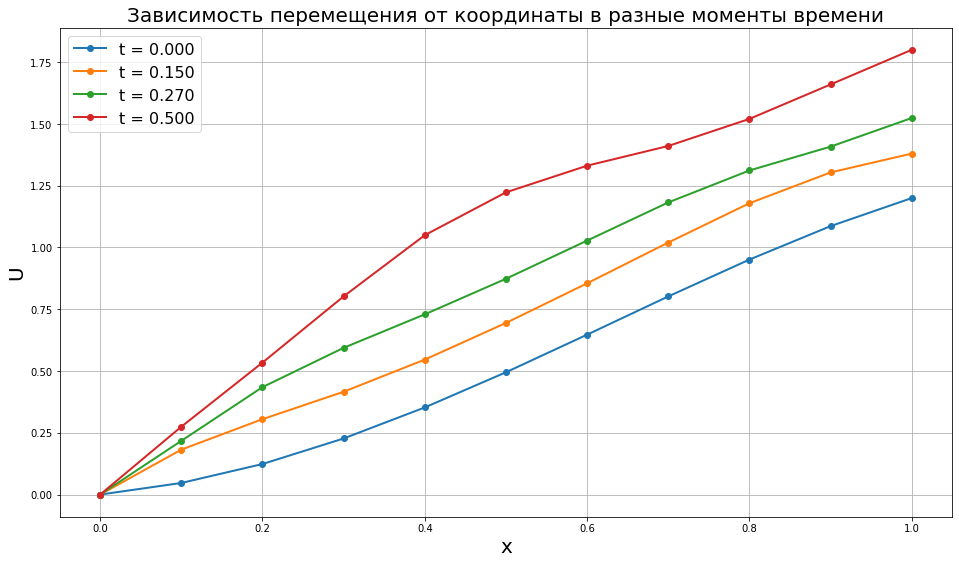
\includegraphics[scale=0.5]{pic2.png}}
		\label{pic2}
		\caption{}
	\end{figure}
	
	\newpage
	
	\section{Приложение}
	
	Далее представлен код программы на Python: \\
	
	\lstinputlisting[language=Python]{code.py}
	
	\newpage
	Табличное представление полученного решения:
	
	\begin{table}[h]
		\begin{tabular}{llllllllllll}
			& 0   & 1     & 2     & 3     & 4     & 5     & 6     & 7     & 8     & 9     & 10    \\
			0  & 0.0 & 0.047 & 0.124 & 0.227 & 0.353 & 0.495 & 0.647 & 0.802 & 0.951 & 1.086 & 1.2   \\
			1  & 0.0 & 0.057 & 0.134 & 0.238 & 0.364 & 0.508 & 0.661 & 0.817 & 0.967 & 1.104 & 1.212 \\
			2  & 0.0 & 0.068 & 0.145 & 0.249 & 0.376 & 0.52  & 0.674 & 0.832 & 0.984 & 1.122 & 1.224 \\
			3  & 0.0 & 0.078 & 0.156 & 0.261 & 0.388 & 0.533 & 0.688 & 0.846 & 1.0   & 1.139 & 1.236 \\
			4  & 0.0 & 0.089 & 0.167 & 0.272 & 0.4   & 0.546 & 0.702 & 0.861 & 1.016 & 1.156 & 1.248 \\
			5  & 0.0 & 0.099 & 0.179 & 0.284 & 0.413 & 0.559 & 0.716 & 0.876 & 1.031 & 1.173 & 1.26  \\
			6  & 0.0 & 0.109 & 0.191 & 0.296 & 0.425 & 0.572 & 0.729 & 0.89  & 1.047 & 1.189 & 1.272 \\
			7  & 0.0 & 0.119 & 0.203 & 0.309 & 0.438 & 0.585 & 0.743 & 0.905 & 1.063 & 1.204 & 1.284 \\
			8  & 0.0 & 0.129 & 0.215 & 0.321 & 0.451 & 0.598 & 0.757 & 0.919 & 1.078 & 1.219 & 1.296 \\
			9  & 0.0 & 0.138 & 0.228 & 0.334 & 0.464 & 0.612 & 0.771 & 0.934 & 1.093 & 1.233 & 1.308 \\
			10 & 0.0 & 0.147 & 0.24  & 0.347 & 0.477 & 0.625 & 0.785 & 0.948 & 1.108 & 1.246 & 1.32  \\
			11 & 0.0 & 0.155 & 0.253 & 0.361 & 0.491 & 0.639 & 0.799 & 0.963 & 1.123 & 1.259 & 1.332 \\
			12 & 0.0 & 0.163 & 0.266 & 0.374 & 0.504 & 0.653 & 0.813 & 0.977 & 1.137 & 1.271 & 1.344 \\
			13 & 0.0 & 0.17  & 0.279 & 0.388 & 0.518 & 0.667 & 0.827 & 0.992 & 1.151 & 1.282 & 1.356 \\
			14 & 0.0 & 0.176 & 0.292 & 0.402 & 0.532 & 0.68  & 0.841 & 1.006 & 1.165 & 1.293 & 1.368 \\
			15 & 0.0 & 0.182 & 0.305 & 0.416 & 0.546 & 0.695 & 0.855 & 1.02  & 1.179 & 1.304 & 1.38  \\
			16 & 0.0 & 0.187 & 0.318 & 0.431 & 0.561 & 0.709 & 0.869 & 1.034 & 1.192 & 1.314 & 1.392 \\
			17 & 0.0 & 0.192 & 0.33  & 0.445 & 0.575 & 0.723 & 0.883 & 1.048 & 1.205 & 1.323 & 1.404 \\
			18 & 0.0 & 0.196 & 0.343 & 0.46  & 0.59  & 0.738 & 0.898 & 1.062 & 1.218 & 1.332 & 1.416 \\
			19 & 0.0 & 0.199 & 0.355 & 0.475 & 0.605 & 0.752 & 0.912 & 1.076 & 1.23  & 1.341 & 1.428 \\
			20 & 0.0 & 0.203 & 0.366 & 0.489 & 0.62  & 0.767 & 0.926 & 1.09  & 1.242 & 1.35  & 1.44  \\
		\end{tabular}
		\caption{U(t,x)}
	\end{table}
	
\end{document}